\section{Architettura Front end}{
	\subsection{com.apim.client}{
		\subsubsection{Informazioni sul package}{
			\begin{figure}[ht]
				\centering
				\includegraphics[width=0.7\textwidth]{img/client}
				\caption{Schema package client}
			\end{figure}
		Questo package racchiude tutta la parte front-end dell'applicazione.
		}
		\subsubsection {Package contenuti}{
			\begin{itemize}
				\item *.model;
				\item *.view;
				\item *.modelView.
			\end{itemize}
		}
	}
	\subsection{com.apim.client.view}{
		\subsubsection{Informazioni sul package}{
			\begin{figure}[ht]
				\centering
				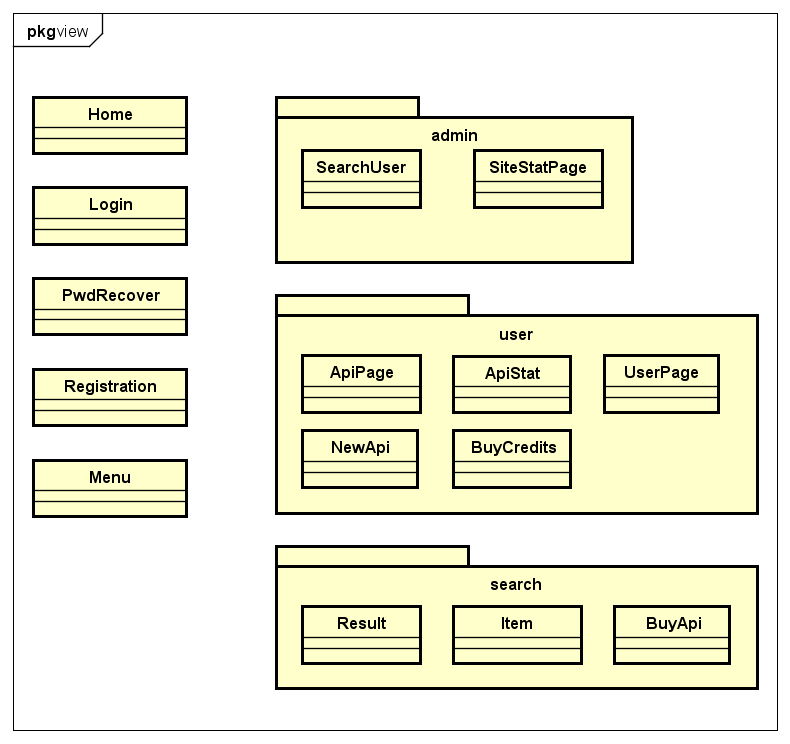
\includegraphics[width=0.7\textwidth]{img/feview}
				\caption{Schema package client - view}
			\end{figure}
		}
		\subsubsection{Package contenuti}{
			\begin{itemize}
				\item com.apim.client.view.user;
				\item com.apim.client.view.search;
				\item com.apim.client.view.admin.
			\end{itemize}
		}
		\subsubsection{Interazione con altri componenti}{
			\begin{itemize}
				\item com.apim.client.modelView;
			\end{itemize}
		}
		\subsubsection{Classi}{
			\begin{itemize}
				\item \textbf{Home}
					\begin{itemize}
						\item \textbf{Descrizione:}  template HTML che forma la pagina principale dell'applicazione.
						\item \textbf{Relazioni con altre classi:}
						\begin{itemize}
							\item com.apim.client.viewModel.navigation.ShowHome.
						\end{itemize}
					\end{itemize}
				\item \textbf{Login}
					\begin{itemize}
						\item \textbf{Descrizione:}  template HTML che compone la pagina di login.
						\item \textbf{Relazioni con altre classi:}
						\begin{itemize}
							\item com.apim.client.viewModel.navigation.ShowLogin.
						\end{itemize}
					\end{itemize}
				\item \textbf{pwdRecover}
					\begin{itemize}
						\item \textbf{Descrizione:}  template HTML che compone la pagina per il recupero della password.
						\item \textbf{Relazioni con altre classi:}
						\begin{itemize}
							\item com.apim.client.viewModel.navigation.ShowRecovery.
						\end{itemize}
					\end{itemize}
				\item \textbf{Registration}
					\begin{itemize}
						\item \textbf{Descrizione:}  template HTML che forma la pagina per la registrazione al sistema.
						\item \textbf{Relazioni con altre classi:}
						\begin{itemize}
							\item com.apim.client.viewModel.navigation.ShowRegistration.
						\end{itemize}
					\end{itemize}
				\item \textbf{Menu}
					\begin{itemize}
						\item \textbf{Descrizione:}  template HTML del menu dell'applicazione.
						\item \textbf{Relazioni con altre classi:}
						\begin{itemize}
							\item com.apim.client.viewModel.navigation.ShowMenu.
						\end{itemize}
					\end{itemize}
			\end{itemize}
		}
	}
	\subsection{com.apim.client.view.user}{
		\subsubsection{Informazione sul package}{
			Questo package contiene i template html relativi alle pagine a cui può accedere un utente che ha già effettuato login.
		}
		\subsubsection{Interazione con altri componenti}{
			\begin{itemize}
				\item com.apim.client.modelView;
			\end{itemize}
		}
		\subsubsection{Classi}{
			\begin{itemize}
				\item \textbf{ApiPage}
					\begin{itemize}
						\item \textbf{Descrizione:} contiene i template html relativi alla pagina delle API registrate dall'utente.
						\item \textbf{Relazioni con altre classi:}
						\begin{itemize}
							\item com.apim.client.viewModel.user.ShowApiPage;
						\end{itemize}
					\end{itemize}
				\item \textbf{ApiStat}
					\begin{itemize}
						\item \textbf{Descrizione:} contiene i template html relativi alla pagina delle statistiche di un'API registrata dall'utente.
						\item \textbf{Relazioni con altre classi:}
						\begin{itemize}
							\item com.apim.client.viewModel.user.ShowApiStat;
						\end{itemize}
					\end{itemize}
				\item \textbf{UserPage}
					\begin{itemize}
						\item \textbf{Descrizione:} contiene i template html relativi alla pagina principale dell'utente registrato.
						\item \textbf{Relazioni con altre classi:}
						\begin{itemize}
							\item com.apim.client.viewModel.user.ShowUserPage;
						\end{itemize}
					\end{itemize}
				\item \textbf{NewAPI}
					\begin{itemize}
						\item \textbf{Descrizione:} contiene i template html relativi alla pagina che permette all'utente registrato di registrare una nuova API.
						\item \textbf{Relazioni con altre classi:}
						\begin{itemize}
							\item com.apim.client.viewModel.user.ShowNewApi;
						\end{itemize}
					\end{itemize}
				\item \textbf{Credits}
				\begin{itemize}
					\item \textbf{Descrizione:} contiene i template html relativi alla pagina che permette all'utente registrato di aggiungere APICredits al suo account.
					\item \textbf{Relazioni con altre classi:}
					\begin{itemize}
						\item com.apim.client.viewModel.user.ShowBuyCredits;
					\end{itemize}
				\end{itemize}
			\end{itemize}
		}
	}
	\subsection{com.apim.client.view.search}{
		\subsubsection{Informazione sul package}{
			Questo package contiene i template html relativi alla ricerca.
		}
		\subsubsection{Interazione con altri componenti}{
			\begin{itemize}
				\item com.apim.client.viewModel;
			\end{itemize}
		}
		\subsubsection{Classi}{
			\begin{itemize}
				\item \textbf{Result}
					\begin{itemize}
						\item \textbf{Descrizione:} Classe che contiene il template html della pagina dei risultati di ricerca.
						\item \textbf{Relazioni con altre classi:}
							\begin{itemize}
								\item com.apim.client.viewModel.navigation.showSearch;
							\end{itemize}
					\end{itemize}
				\item \textbf{Item}
					\begin{itemize}
						\item \textbf{Descrizione:} Classe che contiene il template html della pagina di un API pubblicata.
						\item \textbf{Relazioni con altre classi:}
							\begin{itemize}
								\item com.apim.client.viewModel.navigation.showItemSearch;
								\item com.apim.client.viewModel.navigation.showItemComments;
							\end{itemize}
					\end{itemize}	
				\item \textbf{BuyApi}
					\begin{itemize}
						\item \textbf{Descrizione:} Classe che contiene il template html della pagina di acquisto di una APIKey.
						\item \textbf{Relazioni con altre classi:}
						\begin{itemize}
							\item com.apim.client.viewModel.navigation.showItemBuy;
						\end{itemize}
					\end{itemize}	
			\end{itemize}
		}
	}
	\subsection{com.apim.client.view.admin}{
		\subsubsection{Informazione sul package}{
			Questo package contiene i template html per le pagine relative all'admin.
		}
		\subsubsection{Classi}{
			\begin{itemize}
				\item \textbf{SearchUser}
					\begin{itemize}
						\item \textbf{Descrizione:} Classe che contiene il template html della pagina dei risultati di ricerca utenti.
						\item \textbf{Relazioni con altre classi:}
						\begin{itemize}
							\item com.apim.client.viewModel.admin.showUserSearch;
						\end{itemize}
					\end{itemize}
				\item \textbf{SiteStatPage}
					\begin{itemize}
						\item \textbf{Descrizione:} Classe che contiene il link html alla pagina di Analytics delle statistiche del sito.
						\item \textbf{Relazioni con altre classi:}
						\begin{itemize}
							\item com.apim.client.viewModel.admin.ShowStatPage;
						\end{itemize}
					\end{itemize}	
			\end{itemize}
		}
	}
	\subsection{com.apim.client.model}{
		\subsubsection{Informazione sul package}{
			\begin{figure}[ht]
				\centering
				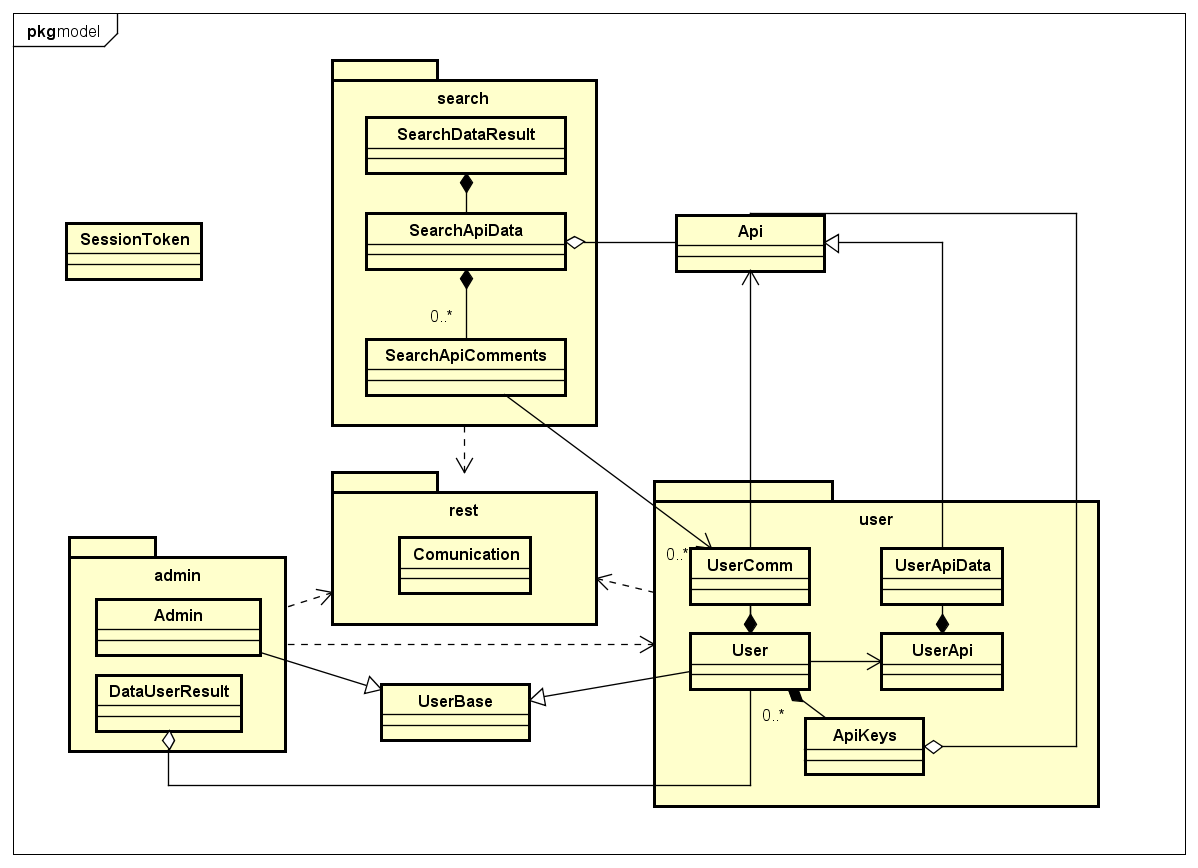
\includegraphics[width=0.7\textwidth]{img/femodel}
				\caption{Schema package client - model}
			\end{figure}
		Questo package contiene il model dell'interfaccia dell'applicazione web, ovvero le classi che importano i dati dal back-end, e salvano i dati inseriti e modificati dall'utente.
		}
		\subsubsection{Package contenuti}{
			\begin{itemize}
				\item com.apim.client.model.search;
				\item com.apim.client.model.user;
				\item com.apim.client.model.admin.
			\end{itemize}
		}
		\subsubsection{Interazione con altri componenti}{
			\begin{itemize}
				\item com.apim.client.modelView.
			\end{itemize}
		\subsubsection{Classi}
			\begin{itemize}
				\item \textbf{SessionToken}
					\begin{itemize}
						\item \textbf{Descrizione:} Questa classe contiene il token che memorizza la sessione dell'utente.
					\end{itemize}
				\item \textbf{Api}
					\begin{itemize}
						\item \textbf{Descrizione:} Questa classe contiene le informazioni pubbliche di una API registrata sul sistema da un utente.
						\item \textbf{Relazioni con altre classi:}
						\begin{itemize}
							\item com.apim.client.model.SearchApiData;
							\item com.api.client.model.UserApiData.
						\end{itemize}
					\end{itemize}
				\item \textbf{UserBase}
					\begin{itemize}
						\item \textbf{Descrizione:} Questa classe contiene le informazioni base in comune tra utenti registrati e utenti admin.
						\item \textbf{Relazioni con altre classi:}
						\begin{itemize}
							\item com.apim.client.model.User;
							\item com.api.client.model.Admin.
						\end{itemize}
					\end{itemize}
			\end{itemize}
		}
	}
	\subsection{com.apim.client.search}{
		\subsubsection{Informazione sul package}{
			Questo package contiene le informazioni relative all'ultima ricerca effettuata dall' utente.
		}
		\subsubsection{Interazione con altri componenti}{
			\begin{itemize}
				\item com.apim.client.model.rest.
			\end{itemize}
			\subsubsection{Classi}{
				\begin{itemize}
					\item \textbf{SearchDataResult}
						\begin{itemize}
							\item \textbf{Descrizione:} Questa classe contiene l'elenco dei risultati dell'ultima ricerca effettuata dall'utente.
							\item \textbf{Relazioni con altre classi:}
							\begin{itemize}
								\item com.apim.client.model.search.SearchApiData;
							\end{itemize}
						\end{itemize}
					\item \textbf{SearchApiData}
						\begin{itemize}
							\item \textbf{Descrizione:} Questa classe contiene un riferimento ad un oggetto Api, e mette in relazione l'API con i commenti scritti dagli utenti.
							\item \textbf{Relazioni con altre classi:}
							\begin{itemize}
								\item com.apim.client.model.search.SearchApiComments;
							\end{itemize}
						\end{itemize}
					\item \textbf{SearchApiComments}
						\begin{itemize}
							\item \textbf{Descrizione:} Questa classe contiene tutti i commenti degli utenti relativi ad un API.
							\item \textbf{Relazioni con altre classi:}
							\begin{itemize}
								\item com.apim.client.model.search.SearchApiData.
								\item com.api.client.model.user.UserComm
							\end{itemize}
						\end{itemize}
				\end{itemize}
			}
		}
	}
	\subsection{com.apim.client.model.user}{
		\subsubsection{Informazione sul package}{
			Questo package contiene le informazioni relative all'utente.
		}
		\subsubsection{Interazione con altri componenti}{
			\begin{itemize}
				\item com.apim.client.model.rest.
			\end{itemize}
			\subsubsection{Classi}
			\begin{itemize}
				\item \textbf{User}
				\begin{itemize}
					\item \textbf{Descrizione:} Contiene i dati personali relativi all'utente.
					\item \textbf{Relazioni con altre classi:}
					\begin{itemize}
						\item com.apim.client.model.user.UserComm;
						\item com.apim.client.model.user.UserApi;
						\item com.apim.client.model.user.ApiKeys.
					\end{itemize}
				\end{itemize}
				\item \textbf{UserComm}
					\begin{itemize}
						\item \textbf{Descrizione:} Contiene tutti i commenti scritti dall'utente.
						\item \textbf{Relazioni con altre classi:}
						\begin{itemize}
							\item com.apim.client.model.Api;
						\end{itemize}
					\end{itemize}
				\item \textbf{UserApi}
					\begin{itemize}
						\item \textbf{Descrizione:} Contiene l'elenco delle API registrate dall'utente.
						\item \textbf{Relazioni con altre classi:}
						\begin{itemize}
							\item com.apim.client.model.user.UserApiData.
						\end{itemize}
					\end{itemize}
				\item \textbf{UserApiData}
					\begin{itemize}
						\item \textbf{Descrizione:} Contiene un riferimento ad un Api e i dati aggiuntivi riguardo alle statistiche visibili dal suo proprietario.
						\item \textbf{Relazioni con altre classi:}
						\begin{itemize}
							\item com.apim.client.model.Api;
							\item com.apim.client.model.user.UserApi.
						\end{itemize}
					\end{itemize}
				\item \textbf{ApiKeys}
					\begin{itemize}
						\item \textbf{Descrizione:} Contiene l'elenco delle APIKeys acquistate dall'utente e un riferimento all'Api a cui appartengono.
						\item \textbf{Relazioni con altre classi:}
						\begin{itemize}
							\item com.apim.client.model.Api;
							\item com.apim.client.model.user.User.
						\end{itemize}
					\end{itemize}
			\end{itemize}
		}
	}
	\subsection{com.apim.client.model.admin}{
		\subsubsection{Informazione sul package}{
			QUesto package contiene le informazioni relative ad un utente Admin.
		}
		\subsubsection{Interazione con altri componenti}{
			\begin{itemize}
				\item com.apim.client.model.rest;
				\item com.apim.client.model.admin.
			\end{itemize}
		}
			\subsubsection{Classi}{
			\begin{itemize}
				\item \textbf{Admin}
					\begin{itemize}
						\item \textbf{Descrizione:} Questa classe contiene tutte le informazioni addizionali relative all'utente Admin.
					\end{itemize}
				\item \textbf{DatauserResult}
					\begin{itemize}
						\item \textbf{Descrizione:} Questa classe contiene i risultati 
						\item \textbf{Relazioni con altre classi:}
						\begin{itemize}
							\item com.apim.client.model.user.User.
						\end{itemize}
					\end{itemize}
			\end{itemize}
		}
	}
	\subsection{com.apim.client.model.rest}{
		\subsubsection{Informazione sul package}{
			Questo pacchetto si occupa della comunicazione con il back-end tramite comunicazione rest.
		}
		\subsubsection{Interazione con altri componenti}{
			\begin{itemize}
				\item com.apim.client.model.search;
				\item com.apim.client.model.user;
				\item com.apim.client.model.admin;
			\end{itemize}
			\subsubsection{Classi}{
				\begin{itemize}
					\item \textbf{Comunication}
					\begin{itemize}
						\item \textbf{Descrizione:} Classe che riceve una richiesta da parte delle altre classi, esegue una chiamata al back-end, e restituisce i dati richiesti.
					\end{itemize}
				\end{itemize}
			}
		}
	}
	\subsection{com.apim.client.modelView}{
		\subsubsection{Informazione sul package}{
			\begin{figure}[ht]
				\centering
				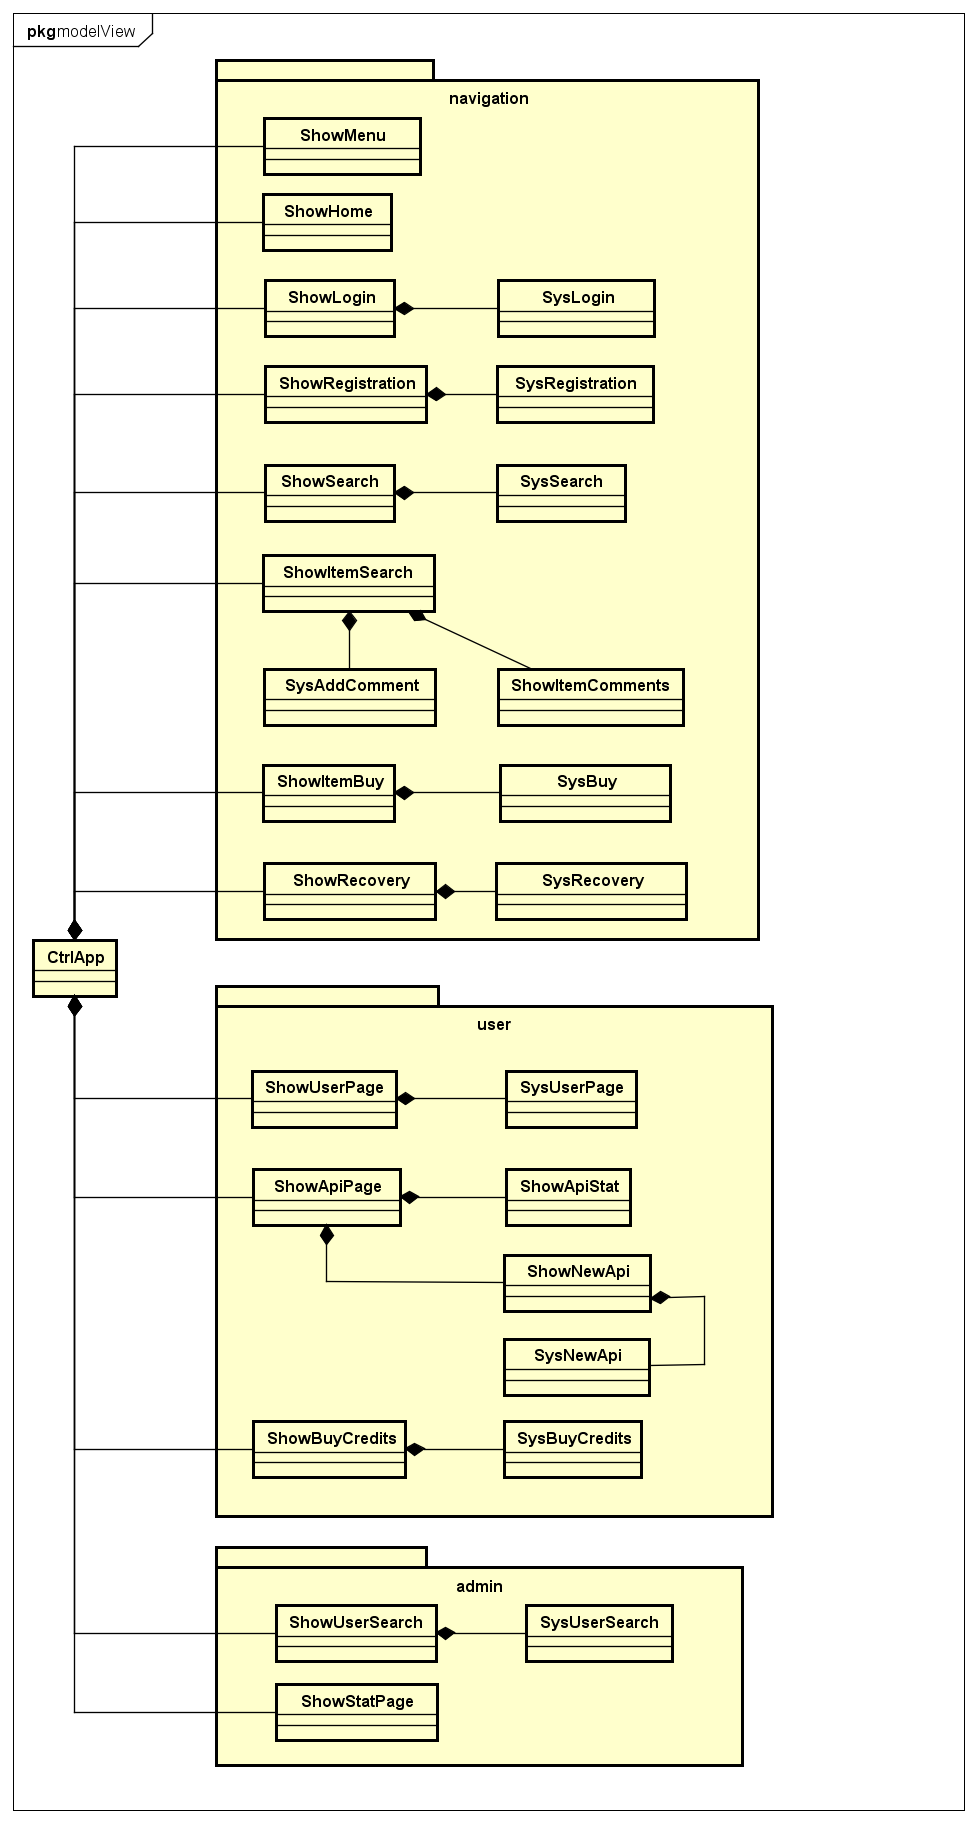
\includegraphics[width=0.7\textwidth]{img/femodelview}
				\caption{Schema package client - modelView}
			\end{figure}
			Questo package si occupa di far comunicare model e view, aggiornando costantemente la view ad ogni cambiamento del model e viceversa.
		}
		\subsubsection{Package contenuti}{
			\begin{itemize}
				\item com.apim.client.modelView.navigation;
				\item com.apim.client.modelView.user;
				\item com.apim.client.modelView.admin;
			\end{itemize}
		}
		\subsubsection{Interazione con altri componenti}{
			\begin{itemize}
				\item com.apim.client.view;
				\item com.apim.client.controller.
			\end{itemize}
			\subsubsection{Classi}
			\begin{itemize}
				\item \textbf{CtrlApp}
				\begin{itemize}
					\item \textbf{Descrizione:} Questa classe si occupa di gestire in modo centralizzato l'applicazione web, ricevendo segnali dalla view e dal model e dirottandolo al componente interessato.
					\item \textbf{Relazioni con altre classi:}
					\begin{itemize}
						\item com.apim.client.modelView.ShowHome;
						\item com.apim.client.modelView.ShowMenu;
						\item com.apim.client.modelView.ShowLogin;
						\item com.apim.client.modelView.ShowRegistration;
						\item com.apim.client.modelView.ShowSearch;
						\item com.apim.client.modelView.ShowItemSearch;
						\item com.apim.client.modelView.ShowItemBuy;
						\item com.apim.client.modelView.ShowRecovery;
						\item com.apim.client.modelView.ShowUserPage;
						\item com.apim.client.modelView.ShowApiPage;
						\item com.apim.client.modelView.ShowBuyCredits;
						\item com.apim.client.modelView.ShowUserSearch;
						\item com.apim.client.modelView.ShowStatPage.
					\end{itemize}
				\end{itemize}
			\end{itemize}
		}
	}
	\subsection{com.apim.client.modelView.navigation}{
		\subsubsection{Informazione sul package}{
			Questo package si occupa della gestione delle pagine di navigazione dell'applicazione: homepage, ricerca e descrizione dei risultati della ricerca.
		}
		\subsubsection{Classi}{
			\begin{itemize}
				\item \textbf{ShowHome}
					\begin{itemize}
						\item \textbf{Descrizione:} Questa classe si occupa di creare la pagina home riempiendo il template sulla view.
						\item \textbf{Relazioni con altre classi:}
							\begin{itemize}
								\item com.apim.client.view.Home;
								\item com.apim.client.model.rest.Comunication;
								\item com.api.client.model.Api.
							\end{itemize}
					\end{itemize}
				\item \textbf{ShowMenu}
					\begin{itemize}
						\item \textbf{Descrizione:} Questa classe si occupa di creare il menu di navigazione.
						\item \textbf{Relazioni con altre classi:}
							\begin{itemize}
								\item com.apim.client.view.Menu;
								\item com.apim.client.model.SessionToken.
							\end{itemize}
					\end{itemize}
				\item \textbf{ShowLogin}
					\begin{itemize}
						\item \textbf{Descrizione:} Classe che crea la pagina di login.
						\item \textbf{Relazioni con altre classi:}
							\begin{itemize}
								\item com.apim.client.view.Login;
								\item com.apim.client.modelView.navigation.SysLogin.
							\end{itemize}
					\end{itemize}
				\item \textbf{SysLogin}
					\begin{itemize}
						\item \textbf{Descrizione:} Classe che esegue il login e restituisce il risultato dell'operazione.
						\item \textbf{Relazioni con altre classi:}
							\begin{itemize}
								\item com.apim.client.model.rest.Comunication;
								\item com.apim.client.model.SessionToken.
							\end{itemize}
					\end{itemize}
				\item \textbf{ShowRegistration}
					\begin{itemize}
						\item \textbf{Descrizione:} Classe che visualizza la pagina di registrazione
						\item \textbf{Relazioni con altre classi:}
							\begin{itemize}
								\item com.apim.client.view.Registration;
								\item com.apim.client.modelView.navigation.SysRegistration.
							\end{itemize}
					\end{itemize}
				\item \textbf{SysRegistration}
					\begin{itemize}
						\item \textbf{Descrizione:} Classe che sottopone la registrazione al server e restituisce il risultato dell'operazione
						\item \textbf{Relazioni con altre classi:}
							\begin{itemize}
								\item com.apim.client.model.rest.Comunication;
								\item com.apim.client.model.SessionToken.
							\end{itemize}
					\end{itemize}
				\item \textbf{ShowSearch}
					\begin{itemize}
						\item \textbf{Descrizione:} Classe che visualizza i risultati di una ricerca effettuata dall'utente.
						\item \textbf{Relazioni con altre classi:}
							\begin{itemize}
								\item com.apim.client.search.result;
								\item com.apim.client.modelView.navigation.SysSearch.
							\end{itemize}
					\end{itemize}
				\item \textbf{SysSearch}
					\begin{itemize}
						\item \textbf{Descrizione:} Classe che esegue la ricerca.
						\item \textbf{Relazioni con altre classi:}
							\begin{itemize}
								\item com.apim.client.model.search.SearchDataResult;
								\item com.apim.client.model.search.SearchApiData.
							\end{itemize}
					\end{itemize}
				\item \textbf{ShowItemSearch}
					\begin{itemize}
						\item \textbf{Descrizione:} Classe che visualizza la pagina di una API ricercata dall'utente.
						\item \textbf{Relazioni con altre classi:}
							\begin{itemize}
								\item com.apim.client.view.search.Item;
								\item com.apim.client.model.search.SearchApiData;
								\item com.apim.client.modelView.SysAddComment;
								\item com.apim.client.modelView.navigation.ShowItemComments.
							\end{itemize}
					\end{itemize}
				\item \textbf{SysAddComment}
					\begin{itemize}
						\item \textbf{Descrizione:} Classe che esegue il controllo e l'inserimento di un nuovo commento.
						\item \textbf{Relazioni con altre classi:}
							\begin{itemize}
								\item com.apim.client.model.SessionToken;
								\item com.apim.client.model.rest.Comunication;
								\item com.apim.client.model.user.User.
							\end{itemize}
					\end{itemize}
				\item \textbf{ShowItemComments}
					\begin{itemize}
						\item \textbf{Descrizione:} Classe che visualizza i commenti relativi all'API visualizzata.
						\item \textbf{Relazioni con altre classi:}
							\begin{itemize}
								\item com.apim.client.model.search.SearchApiComments.
							\end{itemize}
					\end{itemize}
				\item \textbf{ShowItemBuy}
					\begin{itemize}
						\item \textbf{Descrizione:} Classe che visualizza la pagina di acquisto di una APIKey per una API ricercata.
						\item \textbf{Relazioni con altre classi:}
							\begin{itemize}
								\item com.apim.client.view.user.BuyApi;
								\item com.apim.client.model.rest.Comunication;
								\item com.apim.client.model.SessionToken;
								\item com.apim.client.modelView.navigation.SysBuy.
							\end{itemize}
					\end{itemize}
				\item \textbf{SysBuy}
					\begin{itemize}
						\item \textbf{Descrizione:} Classe che esegue l'acquisto e restituisce il risultato dell'operazione.
						\item \textbf{Relazioni con altre classi:}
							\begin{itemize}
								\item com.apim.client.model.rest.Comunication;
								\item com.apim.client.model.user.User;
							\end{itemize}
					\end{itemize}
				\item \textbf{ShowRecovery}
					\begin{itemize}
						\item \textbf{Descrizione:} Classe che visualizza la pagina di recupero della password.
						\item \textbf{Relazioni con altre classi:}
						\begin{itemize}
							\item com.apim.client.view.PwsRecover;
							\item com.apim.client.modelView.navigation.SysRecovery.
						\end{itemize}
					\end{itemize}
				\item \textbf{SysRecovery}
					\begin{itemize}
						\item \textbf{Descrizione:} Classe che esegue la procedura di recupero password.
						\item \textbf{Relazioni con altre classi:}
						\begin{itemize}
							\item com.apim.client.model.rest.Comunication;
						\end{itemize}
					\end{itemize}
			\end{itemize}
		}
	}
	\subsection{com.apim.client.modelView.user}{
		\subsubsection{Informazione sul package}{
			Questo package si occupa delle pagine riservate all'utente autenticato.
		}
		\subsubsection{Classi}{
			\begin{itemize}
				\item \textbf{ShowUserPage}
					\begin{itemize}
						\item \textbf{Descrizione:} Classe che visualizza la pagina utente.
						\item \textbf{Relazioni con altre classi:}
						\begin{itemize}
							\item com.apim.client.modelView.user.SysUserPage;
							\item com.apim.client.view.user.UserPage;
							\item com.apim.client.model.user.User;
							\item com.apim.client.model.SessionToken.
						\end{itemize}
					\end{itemize}
				\item \textbf{SysUserPage}
					\begin{itemize}
						\item \textbf{Descrizione:} Classe che esegue le modifiche alla pagina utente e ritorna il risultato.
						\item \textbf{Relazioni con altre classi:}
						\begin{itemize}
							\item com.apim.client.model.rest.Comunication;
							\item com.apim.client.model.SessionToken;
						\end{itemize}
					\end{itemize}
				\item \textbf{ShowApiPage}
					\begin{itemize}
						\item \textbf{Descrizione:} Classe che visualizza le API registrate dall'utente.
						\item \textbf{Relazioni con altre classi:}
						\begin{itemize}
							\item com.apim.client.modelView.user.ShowApiStat;
							\item com.apim.client.modelView.user.ShowNewApi;
							\item com.apim.client.view.user.ApiPage;
							\item com.apim.client.model.user.UserApi;
							\item com.apim.client.model.SessionToken.
						\end{itemize}
					\end{itemize}
				\item \textbf{ShowApiStat}
					\begin{itemize}
						\item \textbf{Descrizione:} Classe che visualizza le statistiche relative ad una API registrata dall'utente.
						\item \textbf{Relazioni con altre classi:}
						\begin{itemize}
							\item com.apim.client.view.user.ApiStat;
							\item com.apim.client.model.SessionToken;
							\item com.apim.client.model.user.UserApiData.
						\end{itemize}
					\end{itemize}
				\item \textbf{ShowNewApi}
					\begin{itemize}
						\item \textbf{Descrizione:} Classe che visualizza la pagina che permette all'utente di registrare una nuova API.
						\item \textbf{Relazioni con altre classi:}
						\begin{itemize}
							\item com.apim.client.modelView.user.SysNewApi;
							\item com.apim.client.model.SessionToken;
							\item com.apim.client.view.user.NewApi.
						\end{itemize}
					\end{itemize}
				\item \textbf{SysNewApi}
					\begin{itemize}
						\item \textbf{Descrizione:} Classe che esegue la registrazione della nuova API.
						\item \textbf{Relazioni con altre classi:}
						\begin{itemize}
							\item com.apim.client.model.rest.Comunication;
							\item com.apim.client.model.SessionToken.
						\end{itemize}
					\end{itemize}
				\item \textbf{ShowBuyCredits}
					\begin{itemize}
						\item \textbf{Descrizione:} Classe che visualizza la pagina per l'acquisto di nuovi APICredits da parte dell'utente autenticato.
						\item \textbf{Relazioni con altre classi:}
						\begin{itemize}
							\item com.apim.client.modelView.user.SysBuyCredits;
							\item com.apim.client.view.user.BuyCredits;
							\item com.apim.client.model.SessionToken.
						\end{itemize}
					\end{itemize}
				\item \textbf{SysBuyCredits}
					\begin{itemize}
						\item \textbf{Descrizione:} Classe che esegue l'acquisto di nuovi APICredits.
						\item \textbf{Relazioni con altre classi:}
						\begin{itemize}
							\item com.apim.client.model.SessionToken;
							\item com.apim.client.model.rest.Comunication.
						\end{itemize}
					\end{itemize}
			\end{itemize}
		}
	}
	\subsection{com.apim.client.modelView.admin}{
		\subsubsection{Informazione sul package}{
			Questo package si occupa delle funzionalità fornite all'utente admin.
		}
		\subsubsection{Classi}{
			\begin{itemize}
				\item \textbf{ShowUserSearch}
					\begin{itemize}
						\item \textbf{Descrizione:} Classe che mostra i risultati di ricerca utenti.
						\item \textbf{Relazioni con altre classi:}
						\begin{itemize}
							\item com.apim.client.modelView.admin.SysUserSearch;
							\item com.apim.client.model.SessionToken;
							\item com.apim.client.view.admin.SearchUser.
						\end{itemize}
					\end{itemize}
				\item \textbf{SysUserSearch}
					\begin{itemize}
						\item \textbf{Descrizione:} Classe che esegue la ricerca utenti e fornisce il risultato.
						\item \textbf{Relazioni con altre classi:}
						\begin{itemize}
							\item com.apim.client.model.SessionToken;
							\item com.apim.client.Admin;
							\item com.apim.client.DataUserResult.
						\end{itemize}
					\end{itemize}
				\item \textbf{ShowStatPage}
					\begin{itemize}
						\item \textbf{Descrizione:} Classe che mostra la pagina di statistiche del sito.
						\item \textbf{Relazioni con altre classi:}
						\begin{itemize}
							\item com.apim.client.view..admin.SiteStatPage.
							\item com.apim.client.model.SessionToken.
						\end{itemize}
					\end{itemize}
			\end{itemize}
		}
	}
}